
% Le type de votre document
\documentclass[a4paper,10pt]{article}

% Quelques packages pour le francais, vous pouvez saisir du texte accentué.
\usepackage[utf8]{inputenc}
\usepackage[frenchb]{babel}
\usepackage{verbatim}
% Des trucs biens pour le pdf.
\usepackage{ae}
\usepackage{aeguill}
\usepackage[bookmarks=true,colorlinks,linkcolor=blue]{hyperref}
\usepackage{algorithmic}
\usepackage{amsmath,amssymb,mathrsfs}
\usepackage{makeidx}
\usepackage{slashbox}


% Pour inclure des graphiques.
\usepackage{graphicx}

\usepackage{tikz}
\usepackage{pgfplots}


% Pour faire déborder les cases d'un tableau sur plusieurs lignes.
\usepackage{multirow}

\usepackage{geometry}

\usepackage[final]{pdfpages}

\usepackage[french]{algorithme}

%\geometry{top=3cm, bottom=3cm, left=2.5cm, right=2.5cm}

\newtheorem{definition}{Définition}
\newtheorem{proposition}{Proposition}

\begin{document}

%
\includepdf[pages=1]{./couverture.pdf}
%
\includepdf[pages=1]{./nonPlagiat.pdf}
%
%\section*{\begin{center}Remerciements\end{center}}
%\par Tout d'abord, je tiens à remercier Frédéric LARDEUX et Frédéric SAUBION pour leur écoute, leurs disponibilités et leurs explications et pour la liberté qu'ils m'ont laissé lors de la réalisation de ce projet.
%\par Je remercie également les membres du LERIA\footnote{Laboratoire d'études et de recherche en informatique d'Angers}, pour m'avoir accordé leur confiance en m'attribuant ce stage.
%\par Je remercie l'équipe enseignante du DAEU\footnote{Diplôme d'accès aux études universitaire} d'Angers, et particulièrement Eric SCHRAFSTETTER qui m'a mis le pied à l'étrier pour intégrer la faculté des sciences d'Angers.
%\par Enfin, je remercie ma famille, qui m'a toujours soutenu dans la reprise de mes études, et tout particulièrement Lucie, Marius et Paulin qui partagent mes humeurs et mon quotidien.
%
%
%\newpage
%\null
%\begin{flushright}
%\vspace{\fill}
%\textbf{À Marius et Paulin.}
%\vspace{\fill}
%\end{flushright}


\section*{Introduction}
\subsection*{Sujet du stage}
\par La plupart des bactéries appartenant au genre Xanthomonas sont responsables de pathologies sur
une large gamme de cultures économiquement importantes, induisant notamment des pertes
de rendement et diminuant ainsi la valeur marchande des semences. Quelques graines
contaminées suffisent à générer une source d'inoculation primaire et à occasionner ainsi une
dissémination ultérieure plus large. En particulier, le pathovar phaseoli de Xanthomonas axonopodis
(Xap) qui regroupe toutes les souches identifiées comme pathogènes sur le haricot n'est pas
endémique en Europe mais pour limiter son introduction, il est inscrit sur la liste des agents
pathogènes de quarantaine. Une approche possible pour l'identification des souches bactériennes
consiste à utiliser un répertoire de gènes de virulence. Il s'agit ainsi de trouver la plus petite
combinaison de gènes de virulence spécifiques. Cette combinaison peut ainsi être utilisée pour
concevoir un test d'identification. Des travaux préliminaires[CHHEL et al.2013] montrent que la combinaison des
tests moléculaires ainsi obtenus fournit une technique rapide pour l'identification de toutes les
souches de Xanthomonas pathogènes sur les haricots.
\par Avec les possibilités accrues d'acquisition de données génomiques – par exemple le séquençage à
haut débit – mais également phénotypiques, le problème de la caractérisation de données
biologiques devrait rapidement devenir l'un des verrous essentiel de l'exploitation effective des
grandes bases de données qui sont en cours de constitution, et constituera donc un centre d'intérêt
commun aux biologistes des domaines du végétal ou de la santé. La caractérisation telle que nous
l'entendons permet d'identifier les caractères propres, éventuellement hétérogènes, d'un groupe
d’individus partageant des spécificités fonctionnelles communes (par exemple pathologiques).
\par Du point de vue informatique, ce problème est abordé comme la recherche d'un ensemble de
formules propositionnelles (variables booléennes) permettant de caractériser de manière exacte les
groupes de pathogènes. Les algorithmes mis en jeu reposent sur des explorations arborescentes
(Branch \& Bound) et des algorithmes heuristiques (recherche locale).
\par L'objectif de ce stage est double :
\begin{itemize}
\item D'une part il s'agit de constituer de nouveaux jeux de données, en dialogue avec nos collègues
biologistes. Ceci requiert la définition de formats et l'exploration de base de données pour la collecte
d'informations pertinentes. Ce travail sera effectué en lien étroit avec les laboratoires de l'INRA
Angers.
\item D'autre part, il s'agit également d'améliorer les algorithmes existants et de proposer de nouvelles
approches pour traiter des instances de grande taille. Cette phase s'inspire des algorithmes de
résolution de problèmes combinatoires (SAT-CSP).
\end{itemize}

\subsection*{Plan du mémoire}
Dans la première partie de ce mémoire, nous dressons un état de l'art concernant l'étude du MIN-PCM, ensuite nous décrivons les contributions que nous apportons à l'étude de ce problème: nous définissons la notion d'instance difficile, nous proposons des heuristiques de résolution (exactes ou approchées) et nous fournissons les résultats ainsi obtenus.\textit{[Ici, peut etre la génération d'instance difficile].} Enfin, nous tirons les conclusions de nos travaux et nous discutons les perspectives de recherche envisagées\textit{[à court et à long terme]}.

% La table des matières
\newpage
\tableofcontents
\newpage

\section{État de l'art}

\subsection{Notations}
Dans ce mémoire, nous utilisons les notations suivantes:
\begin{itemize}
\item $\mathcal{X}$ représente l'ensemble des gènes d'une instance non redondante.
\item $\mathcal{G}$ représente l'ensemble des gènes d'une instance non redondante.
\item $\mathcal{E}$ représente l'ensemble des gènes d'une instance non redondante.
\item $|\mathcal{X}|$ représente la cardinalité de l'ensemble $\mathcal{X}$.
\item $|\mathcal{G}|$ représente la cardinalité l'ensemble $\mathcal{G}$.
\item $|\mathcal{E}|$ représente la cardinalité l'ensemble $\mathcal{E}$.
\end{itemize}

\subsection{Présentation du problème}
\subsubsection*{Problème de caractérisation multiple}
Reprise des définitions présente dans l'article [CHHEL et al.2013](voir si cela est possible)
\subsubsection*{Minimisation du problème de caractérisation multiple}
La minimisation du problème de caractérisation multiple consiste à définir le plus petit nombre de gène pouvant caractériser une instance PCM.
\subsection{Complexité}
Le problème SET-COVER appartient à la classe de complexité W[2]-complet. Il a été montré dans [CHHEL et al.2013] qu'une instance PCM pouvait être réduite en temps polynômial en une instance SET-COVER. Il en résulte que PCM appartient à la classe de complexité W[2]-complet \footnote{En admettant l'hypothèse que la WEFT-hiérarchie proposé par [Downey, Fellows, 1995] soit correcte.}. Dès lors, il a été prouvé que le MIN-PCM appartient à la classe de complexité W[2]-difficile. L'impact direct de l'appartenance de MIN-PCM à cette classe de complexité est que l'\textbf{unique} possibilité d'améliorier significativement la résolution complète\footnote{Recherche exacte permettant de prouver l'optimalité d'une solution.} d'une instance est de \textbf{travailler sur des heuristiques de choix de variables}(gènes). 

\subsection{Une résolution basés sur les fonctions booléenes partiellement définis}
\subsubsection{Résolution complète : Exact-Proj-Car et reformulation en programmation linéaire}
\paragraph{Exact-Proj-Car}
\paragraph{Reformulation en programmation linéaire}
MIN-ONES
\subsubsection{Résolution par recherche locale}
Local-Search-Proj-Car

\subsection{Résultats expérimentaux}
Afin d'avoir un moyen de comparaison pour nos contributions, nous reproduisons ici les résultats fourni dans [CHHEL et al, 2013]\footnote{Nous nous sommes servi du code mis à disposition sur \url{http://forge.info.univ-angers.fr/~gh/Idas/Ccd/mcps/}}. Les expérimentations sont faites sur une machine composé d'un processeur Intel Core\up{tm} i7-2620M CPU à 2.70GHz (deux cœurs) avec 4 Go Ram tournant sous Linux 64-bits. L'option de compilation -Ofast est activé pour obtenir notre exécutable.
\begin{center}
\begin{tabular}{|c|c|c|c|c|c|c|}
\hline 
Instances & Entités(SR) & Groupes & Gènes(SR) & PL & EPC(DIFF)(SH) & LSPC(DIFF) \\ 
\hline 
s301-0 & 500 & 30 & 400 & - & 13 & 14 \\ 
\hline 
s326-0 & 500 & 10 & 500 & - & 13 & 14 \\ 
\hline 
s413-30 & 500 & 20 & 600 & - & 13 & \textcolor{blue}{13} (14) \\ 
\hline 
s555-20 & 800 & 20 & 800 & - & 13 & \textcolor{blue}{13} (14) \\ 
\hline 
s625-20 & 500 & 5 & 1000 & - & 13 & \textcolor{blue}{13} (14) \\ 
\hline 
s754-10 & 600 & 10 & 200 & - & 13 & 14 \\ 
\hline 
s882-20 & 600 & 10 & 400 & - & 13 & 14 \\ 
\hline 
s2501-70 & 800 & 10 & 800 & - & \textcolor{blue}{15} (14) & 15 \\ 
\hline 
s31294-50 & 200 & 15 & 1000 & 10 & 10 & 11 \\ 
\hline 
s3836-0 & 1000 & 15 & 1000 & - & 16 & 16 \\ 
\hline 
raphv & 109 (108) & 8 & 155 (68) & \textbf{6} & \textbf{6} & 9 \\ 
\hline 
raphy & 113 (112) & 4 & 155 (70) & \textbf{6} & \textbf{6} & 8 \\ 
\hline 
rarep & 112 & 7 & 155 (72) & \textbf{12} & 95 (59) (\textcolor{blue}{39}) & 14 \\ 
\hline 
rch8 & 132 (56) & 21 & 37 (27) & \textbf{9} & \textbf{9} & 9 \\ 
\hline 
rch10 & 173 (112) & 27 & 98 (86) & \textbf{10} & 27 (15) (\textcolor{blue}{25}) & 15 \\ 
\hline 
\end{tabular} 
\end{center}
Colonne PL: Résultats obtenu par reformulation en programmation linéaire sur le solveur IBM \textit{cplex}\footnote{\url{http:://www.ibm.com/software/integration/optimization/cplex-optimizer}}.Les instances marqués par "-" ne pas pu être chargé en mémoire car elles solicitaient plus de 32 Go de RAM.\\
SR: Obtenu après suppression des redondances.\\
DIFF: Résultats affichés dans l'article étant différents de ceux obtenus sur notre machine.\\
SH: Résultats obtenu sans heuristique avec notre programme sur notre machine.\\


Les différences significatives sur les instances rarep et rch10 sont du au fait que ces résultats ont été obtenu en partant d'une borne supérieur égale aux nombre de gènes divisé par deux. De fait , il apparaît clairement que l'instance rarep n'a pas bénéficié de la suppression de ses redondances\footnote{$72/2<59$}.

Pour les comparaisons à venir sur les résultats qui diffèrent, nous prendrons en compte les résultats en bleu.

Pour l'instance rch10, le résultat sans heuristique étant meilleur que celui avec l'heuristique de EPC \footnote{Ce qui peut s'expliquer par une différence de structure et d'implémentation du code source.} sur notre machine, nous sommes en mesure de penser que le résultat indiqué dans l'article est erroné, donc nous choisissons de conserver le résultat sans heuristique.



\section{Contributions}

\subsection{Introduction} 
Cette section présente les démarches de recherche qui ont été effectué durant le stage.\\
Dans un premier temps, nous faisons une proposition qui permet d'identifier si une instance est difficile ou non.\\
Ensuite, nous abordons la résolution du problème MIN-PCM avec deux approches différentes :
\begin{itemize}
\item Une recherche exacte qui à la possibilité de prouver la borne minimum du MIN-PCM sur des instances de taille raisonnable.
\item Une recherche approché qui à la possibilité de trouver des solutions de bonne qualité mais non nécessairement optimal en un temps polynômial sur des instance de grande taille.
\end{itemize} 
\textit{TODO: Enfin, nous générons des instances pseudo-aléatoire de différents degrés de difficultés que nous soumettons à nos algorithmes.}

\subsection{Définition d'une instance difficile}
Prenons deux instances: une réelle (rch10) et une aléatoire (s3836-0), voici leurs caractéristiques:
\begin{center}
\begin{tabular}{|c|c|c|c|c|c|}
\hline 
Instances & Entités & Groupes & Gènes & Résolution PL & Résolution EPC\footnote{[Exact-Proj-Car CHHEL et al]} \\ 
\hline 
s3836-0 & 1000 & 15 & 1000 & - & 16 \\ 
\hline
rch10 & 173 & 27 & 98 & \textbf{10}\footnote{En gras = solution optimal} & 14 \\ 
\hline
\end{tabular} 
\end{center}
\vspace{7mm}

A priori, on peut supposer que l'instance aléatoire est plus difficile à résoudre: elle est bien plus volumineuse que l'instance réelle à tel point qu'elle nécessite plus de 32 Go de RAM pour une résolution en programmation linéaire.

Observons leurs résolutions avec notre algorithme sans heuristique:

\begin{figure}[H]
\begin{center}
\begin{tikzpicture}
\begin{axis}[enlarge x limits=false,
xlabel={Caractérisation de taille k},
ylabel={Nombre de comparaisons d'entités},
xmin={14},
xmax={40},
%title={Résolution sans heuristique de rch10 et s3836-0 sur les comparaisons}
]
\addplot +[mark=none] table[x index=0,y index=1]{./resultats/sh_rch10_nbComp};
\addplot +[mark=none] table[x index=0,y index=1]{./resultats/sh_s3836_nbComp};
\end{axis}
\end{tikzpicture}
\end{center}
\caption{Résolution sans heuristique de rch10 et s3836-0 : nombre de comparaisons}
\end{figure}

\begin{figure}[H]
\begin{center}
\begin{tikzpicture}
\begin{axis}[enlarge x limits=false,
xlabel={Caractérisation de taille k},
ylabel={Temps d'éxécution en seconde},
xmin={14},
xmax={40}]
\addplot +[mark=none] table[x index=0,y index=1]{./resultats/sh_rch10_temps};
\addplot +[mark=none] table[x index=0,y index=1]{./resultats/sh_s3836_temps};
\end{axis}
\end{tikzpicture}
\end{center}
\caption{Résolution sans heuristique de rch10 et s3836-0 : temps d'éxécution}
\end{figure}

Nous apercevons que l'instance aléatoire est facilement résolu jusqu'à une caractérisation de taille 15. Ce n'est pas le cas de l'instance réelle qui ne peut plus caractériser en un temps raisonnable à partir d'une caractérisation de taille 25. Ce type d'observation étant \textbf{systématique} quelque soit les caractéristiques des instances réelles ou aléatoire comparés, nous pouvons alors affirmer que la taille d'une instance ne suffit pas à elle seule pour définir sa difficulté. Dès lors, nous nous posons les deux questions suivantes:\\

\begin{itemize}
\item \textbf{Qu'est ce qui peut bien être à l'origine de cette différence de résolution entre une instance aléatoire et une instance réelle?}
\item \textbf{Existe il une méthode permettant de définir si une instance est difficile à résoudre ou non ?}\\
\end{itemize}
Afin de répondre à ces questions, nous définissons les notions suivantes:

\begin{definition}
Le \textbf{masque $M$ d'un groupe $g$} correspond à la moyenne des présences/absences des gènes pour chaque entité du groupe.\\
Formellement, soit $M$ le masque d'un groupe $g \in \mathcal{G}$, $M_i$ la valeur du masque en position $i$, $i \in [1,|\mathcal{X}|]$,
% $|\mathcal{X}|$ étant le nombre de gènes de l'instance après la suppression des redondances,
$$\forall i \in  [1, |\mathcal{X}|], M_i= \frac{\sum_{i=1}^{|\mathcal{G}|}e_i}{|\mathcal{G}|} $$
\end{definition}

\begin{definition}
Le \textbf{ratio $r$ d'un masque $M$} correspond au pourcentage de valeur entière (0/1) présentent dans le masque.\\
Formellement, soit $M$ le masque d'un groupe $g \in \mathcal{G}$, $r_g(I)$ le ratio du groupe $g$ dans l'image $I$,
\begin{center}
$$ r_g(I)=\frac{|{i / M_i \in \{0,1\}}|}{|\mathcal{X}|},\forall i \in [1,|\mathcal{X}|]$$
\end{center}
\end{definition}

\subsubsection*{Exemple :}
\begin{center}
\begin{tabular}{|c|c|c|c|c|c|c|c|c|c|c|}
\hline 
\backslashbox{Entités}{Gènes} & g0 & g1 & g2 & g3 & g4 & g5 & g6 & g7 & g8 & g9 \\ 
\hline 
e1 & 1 & 1 & 0 & 1 & 1 & 1 & 0 & 0 & 0 & 1 \\ 
\hline 
e2 & 1 & 1 & 0 & 1 & 1 & 1 & 0 & 1 & 0 & 1 \\ 
\hline 
e3 & 1 & 1 & 0 & 0 & 0 & 1 & 0 & 0 & 0 & 0 \\ 
\hline 
e4 & 1 & 1 & 0 & 1 & 0 & 1 & 0 & 0 & 0 & 0 \\ 
\hline 
e5 & 1 & 1 & 0 & 1 & 1 & 1 & 0 & 1 & 0 & 0 \\ 
\hline 
\hline
Masque & 1 & 1 & 0 & 0.8 & 0.6 & 1 & 0 & 0.4 & 0 & 0.4 \\
\hline
\end{tabular}
\end{center}
Le ratio $r$ de ce groupe est : \\
$r=6/10$\\
soit  $r=0.6$

\begin{definition}
L'\textbf{image $I$ d'une instance} est une matrice en deux dimensions de taille $|\mathcal{G}|*|\mathcal{X}|$ où chaque ligne correspond au masque de chacun des groupes de l'instance.\\
Formellement, soit $I_i$ la ligne i de la matrice $I$ correspondant à l'image de l'instance $\mathcal{I}$, $M_i$ le masque du groupe $i$ de l'instance $\mathcal{I}$,
$$\forall i \in [1,|\mathcal{G}|], I_i=M_i$$
\end{definition}


\begin{definition}
Le \textbf{taux de similarité globale} $\mathcal{T}_j$ d'un gène $j$ correspond à la moyenne des valeurs de la colonne $j$ sur l'image $I$ d'une instance $\mathcal{I}$.\\
Formellement, soit $I$ l'image d'une instance $\mathcal{I}$, $i$ la $i$\up{ème} ligne de $I$, $j$ la $j$\up{ème} colonne de $I$, $I_{ij}$ est la valeur dans $I$ en ligne $i$ et en colonne $j$, $\mathcal{T}_j(I)$ le taux de similarité globale du gène $j$ dans l'image $I$,
$$ \text{Soit } X=\frac{\sum_{i=1}^{|\mathcal{G}|} I_{ij}}{\mathcal{G}} $$ 
$$\text{Si } X<0.5 \text{ alors } \mathcal{T}_j(I)=(0.5-X)*2 $$
$$\text{sinon }\mathcal{T}_j(I)=(0.5-(1-X))*2$$ 
\end{definition}
Ainsi formuler, $\mathcal{T}_j(I) \in [0,1]$, et, plus le taux de similarité globale d'un gène est élevé, plus sa présence(resp. abscence) dans l'instance est redondante.

\begin{definition}
Le \textbf{coefficient de difficulté $\rho$ d'une instance}, correspond à la moyenne des taux de similarité globaux d'une instance.\\
Formellement, soit $I$ l'image d'une instance $\mathcal{I}$, $j$ la $j$\up{ème} colonne de $I$, $\mathcal{T}_j(I)$ le taux de similarité globale du gène $j$ dans l'image $I$,
$$ \rho=\frac{\sum_{j=1}^{|\mathcal{X}|}\tau_j(I)}{|\mathcal{X}|} $$
\end{definition}

\begin{definition}
Le \textbf{coefficient de difficulté $\sigma$ d'une instance}, correspond à la moyenne des ratios des masques d'une instance.\\
Formellement, soit $I$ l'image d'une instance $\mathcal{I}$, $i$ la $i$\up{ème} ligne de $I$, $r_i(I)$ le ratio du groupe $i$ dans l'image $I$,
$$ \sigma=\frac{\sum_{i=1}^{|\mathcal{G}|}r_i(I)} {|\mathcal{G}|} $$
\end{definition}

Reprenons nos deux instances rch10 et s3836-0 et calculons leurs coefficients de difficultés:

\begin{center}
\begin{tabular}{|c|c|c|}
\hline 
Instances & $\rho$ & $\sigma$ \\ 
\hline 
s3836-0 & 0 & 0.024322 \\ 
\hline
rch10 & 0.906115 & 0.626381 \\ 
\hline
\end{tabular} 
\end{center}

Nous observons que le coefficient de difficulté $\rho$ est plus significatif que $\sigma$, mais nous ne sommes pas en mesure d'indiquer dans quel proportions. Cependant les travaux de [CHHEL et al, 2013] nous indiquent que seul une heuristique sur le choix des variables est en mesure de pouvoir améliorer un algorithme de recherche exacte. Nous pensons donc que $\rho$ a plus d'influence que $\sigma$ sur la difficulté d'une instance. 

\begin{proposition}
Une instance dont le coefficient de difficulté $\rho$ est proche de 1 est une \textbf{instance difficile} à résoudre.
\end{proposition}

\begin{proposition}
Une instance dont le coefficient de difficulté $\rho$ est proche de 1 et dont le coefficient de difficulté $\sigma$ est proche de 0 est une \textbf{instance très difficile} à résoudre.
\end{proposition}

\begin{proposition}
La taille d'une instance (caractérisé par son nombre de gènes et d'entités mais pas son nombre de groupe) est une information sur la difficulté de sa résolution. Cependant cette difficulté est intrinsèque au problème est ne peut pas être réduite de façon significative par un algorithme.
\end{proposition}

%Les observations sur notre jeu de 15 instances nous permettent de conclure que $\sigma$ en particulier, et $\rho$ dans une moindre mesure, nous permettent de définir ce qu'est une instance difficile. 


\subsection{Recherche exacte}
\subsubsection{Introduction}
Nous présentons les heuristiques ayant été mise en place pour la résolution d'instance MIN-PCM. Chaque nouvelle heuristique est ajouté à(aux) précédentes. Les comparaisons se font sur l'instance rch10, entre l'ancienne heuristique la plus puissante connu et la nouvelle mise en place. 

Une comparaison entre la meilleure combinaison d'heuristique trouvé et l'heuristique "CCD" proposé par [CHHEL et al,2013] dans \textit{Exact-Proj-Car} est présenté à la fin de la cette section.
\subsubsection{Heuristique des plus mauvais d'abord (pmda)}
Lorsque nous parcourons une instance pour une caractérisation de taille $k$. On peut affecter un poids sur la paire d'entités comparés deux à deux sur les indices de la combinaison courante.

Formellement, soit $e_a$, $e_z$ deux entités n'appartenant pas au même groupe, $\mathcal{C}$ une combinaison de $\mathcal{C}_{|\mathcal{X}|}^k$, $P$ le poids de la paire $\{e_a,e_z\}$.
$$ P = |\{i / e_a(i)=e_z(i), \forall i \in \mathcal{C}\}| $$

\begin{definition}
Si $P>=k-1$ alors la \textbf{paire d'entités $\{e_a,e_z\}$ est critique} car lors du parcours de la prochaine combinaisons, cette paire à la plus forte probabilité de permettre une coupure dans l'arbre de recherche.
\end{definition}

\subsubsection*{Exemple :}
Soit les 2 entités suivante:
\begin{center}
\begin{tabular}{|c|c|c|c|c|c|c|c|}
\hline 
Groupe & \backslashbox{Entités}{Gènes} & g1 & g2 & g3 & g4 & g5 & g6 \\ 
\hline 
1 & e1 & 1 & 0 & 1 & 0 & 0 & 0 \\ 
\hline 
20 & e400 & 1 & 0 & 0 & 0 & 0 & 1 \\ 
\hline 
\end{tabular}
\end{center}
Supposons que nous sommes dans le cas d'une caractérisation de taille 3, nous parcourons les combinaisons de $\mathcal{C}_6^3 $. Supposons que le groupe 1 soit de taille 1, si nous sommes à la comparaison entre e1 et e400, cela signifie que nous avons déjà effectué 399 comparaisons d'entités. 

Regardons alors la combinaison courante 123 : nous apercevons que seul g3 permet la caractérisation. Comme plusieurs des combinaisons suivantes ne différeront que d'un élément, cet paire d'entités \{e1,e400\} à la plus forte probabilité d'être similiraire lors de la prochaine combinaison, nous gardons donc en mémoire cet ensemble qui a un poids égale à $k-1$.

Supposons que 123 n'ai pas caractérisé notre instance, nous parcourons alors 124 : nous commençons par parcourir les ensembles critiques obtenus lors du parcours précédent, soit la comparaison entre e1 et e400. Le poids est alors égale à $k$, ce qui signifie que nous pouvons arrêter notre recherche sur cette combinaison (car celle ci ne pourra en aucun cas caractériser l'instance). Cependant nous gardons en mémoire cet ensemble critique. Notons que nous avons fait là l'économie de 399 comparaisons d'entités.

Nous parcourons alors 125 : même constat , de nouveau une économie de 399 comparaisons d'entités.

Nous parcourons alors 126 : aucun effet, mais la paire \{e1,e400\} est toujours considérer comme critique.

Nous parcourons alors 134 : aucun effet, mais la paire  \{e1,e400\} n'est plus considéré comme critique car son poids $<k-1$.

\subsubsection*{Résultats}
\begin{figure}[H]
\begin{center}
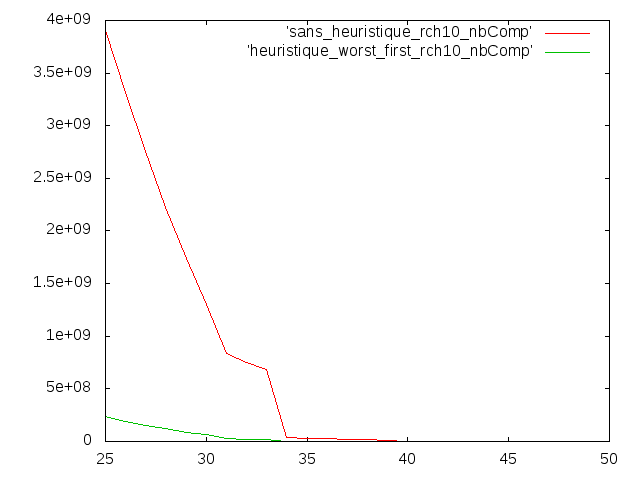
\includegraphics[scale=0.6]{./graphique/diff1_nbComp.png}
\end{center}
\caption{Heuristique 1: Différence sur le nombre de comparaisons effectués}
\end{figure}
\begin{figure}[H]
\begin{center}
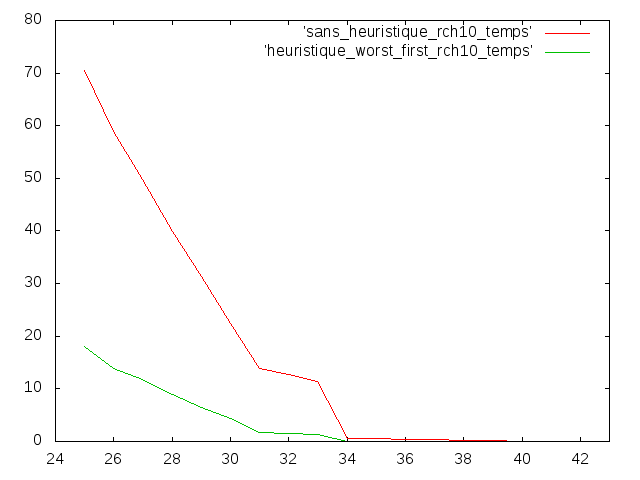
\includegraphics[scale=0.6]{./graphique/diff1_temps.png}
\end{center}
\caption{Heuristique 1: Différence de temps d'exécution}
\end{figure}
On constante que le nombre de comparaisons d'entités ainsi que le temps d'éxécution sont considérablement diminué par l'heuristique.

Ce type de résultat ayant été observé systématiquement sur un jeu de 15 instances(aléatoire et réelle), on peut conclure que cette heuristique est efficace.


\subsubsection{Heuristique par trie de taux de similarité globale $\mathcal{T}$ }
Les outils mis en place pour définir ce qu'est une instance difficile vont maintenant nous permettre d'obtenir de nouvelles heuristique. Dans cette section, nous ordonnons les gènes par ordre croissant sur leur taux de similarité globale $\mathcal{T}$. Dès lors, nous parcourons en priorité les gènes présentant un faible taux de similarité, ce qui a pour effet de caractériser au plus tôt l'instance.

\subsubsection*{Résultats}
\begin{figure}[H]
\begin{center}
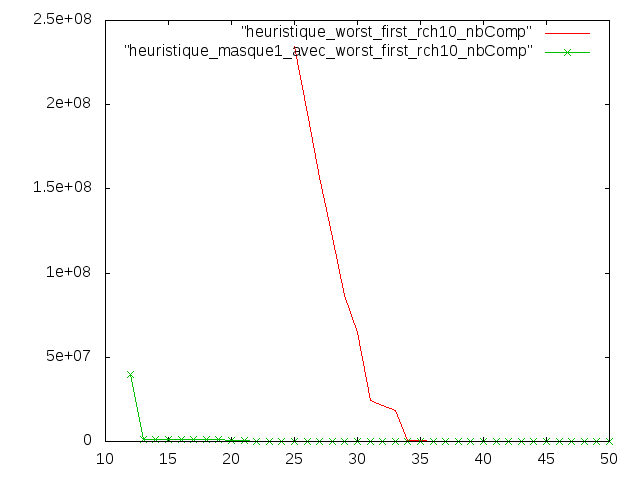
\includegraphics[scale=0.6]{./graphique/diff2_nbComp.png}
\end{center}
\caption{Heuristique 2: Différence sur le nombre de comparaisons effectués}
\end{figure}
\begin{figure}[H]
\begin{center}
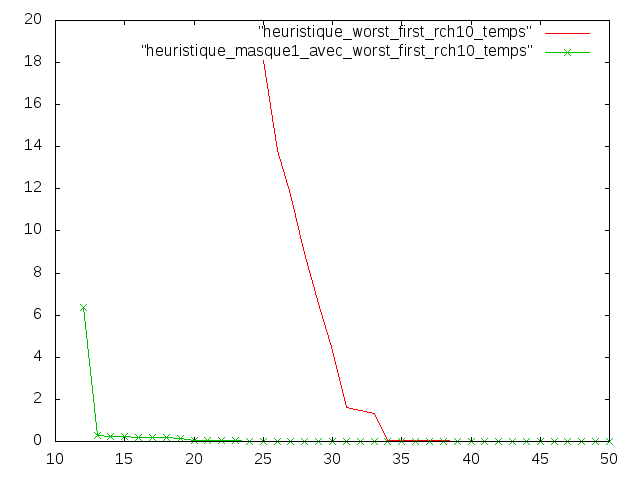
\includegraphics[scale=0.6]{./graphique/diff2_temps.png}
\end{center}
\caption{Heuristique 2: Différence de temps d'exécution}
\end{figure}

On constante que le nombre de comparaisons d'entités est considérablement diminué par l'heuristique. Sans surprise, le temps d'éxécution est également bien plus rapide, d'autant plus que cette heuristique ne coute rien en terme de calcul puisque celui est effectué une seul fois lancement de l'algorithme.

\subsubsection{Heuristique par trie de taux de similarité locale $\tau$}
\subsubsection{Heuristique par trie de ratio $r$}

\subsubsection{Résultats}

\subsection{Recherche incomplète}
\subsubsection{Résultats}

\subsection{Générateur d'instance difficile}
\subsubsection{Résultats}

\section{Conclusions} 

\subsection{Difficultés rencontrées}

\subsection{Conclusions générales}

\subsection{Évolutions possibles et perspective de recherche}
\subsubsection{A court terme}
\subsubsection{A long terme}


\subsection*{\begin{center} Résumé \end{center}}
\addcontentsline{toc}{chapter}{Résumé / Abstract}

\par Ce rapport porte sur la ....
\\\\
\textbf{Mots-clés:} azerty

\subsection*{\huge \begin{center} Abstract \end{center}}

\par This report concerns the ....
\\\\
\textbf{Keywords:} azerty


\end{document}


%\part{État de l'art}
%\chapter{C.S.P. et Q.C.S.P.}
%\par
%C.S.P. signifie \texttt{constraint satisfaction problem}, soit problème de satisfaction de contrainte. Il s'agit en fait d'une formalisation d'un problème sous la forme d'un triplet $\langle X, D, C \rangle$ avec :\\ 
%$X$ : l'ensemble des variables du problème\\
%$D$ : le (les) domaine(s) contraint(s) aux variables de $X$\\ 
%$C$ : l'ensemble des contraintes entre/sur les variables de $X$\\
%
%\par L'apparition de quantificateur universel dans le problème initial peut vite faire exploser ce type de représentation dès que la taille des domaines commence à devenir significative. Alors que, l'universalité est une donnée intrinsèque aux problèmes et que nous savons la gérer au sein même d'une machine de Turing\footnote{En effet, une contrainte sur une variable universelle est respectée si l'ensemble des valeurs du domaine de la variable convient pour la contrainte. Il ne s'agit donc là que d'une énumération classique de toute les valeurs possibles de la variable}. Comme la machine sait gérer ce problème de façon interne, nous nous sommes penchés sur une formalisation plus simple des problèmes pouvant contenir des quantificateurs universelle\footnote{Je rappelle que, bien que cela ne soit pas précisé, le quantificateur existentiel est présent de façon implicite dans les problèmes lorsque ceux-ci sont dépourvus de quantificateur universel}, les Q.C.S.P.\\
% 
%\par
%Q.C.S.P. signifie donc \texttt{quantified constraint satisfaction problem}, soit problème de satisfaction de contraintes quantifiées. La formalisation est la même que pour un C.S.P., à ceci près que les variables sont associées au sigle $\forall$(universelle) ou $\exists$(existentielle)
%
%\chapter{Espace de recherche, paysage}
%\par
%Un espace de recherche est un ensemble contenant(potentiellement, virtuellement) toutes les configurations(combinaisons, individus) possibles des variables d'un problème. Parmi ces configurations figurent donc les solutions du problème et des combinaisons pour lesquelles il reste un certain nombre $N$ de conflits.
%
%\par 
%On peut se faire une idée visuelle d'un tel espace de recherche en le modélisant sur un repère orthonormé avec en abscisse chaque élément de l'espace de recherche et en ordonnée le nombre de conflits $N$ de chaque combinaison. Une telle modélisation est appelée paysage de recherche. Nous pourrions par exemple obtenir:\\
%%\includegraphics{paysage.png}\\
%Source image: \href{http://www.tony-lambert.fr/these/sommaire.html}{Thèse Tony LAMBERT.}\\
%
%\par
%Comme vous pouvez le constater sur l'image ci-dessus, un paysage de recherche peut être constitué de vallées et de collines, plus ou moins hautes et profondes. Nous appelons les creux de vallées les plus profondes les minimums globaux qui correspondent à des solutions du problème et le creux des autres vallées des minimums locaux. Nous reviendrons par la suite sur la signification de ces termes.
%
%\chapter{Solveurs de contraintes}
%\par Un solveur de contrainte est un logiciel qui a pour but de trouver une solution à un C.S.P.. Plusieurs type de recherches sont possibles pour essayer d'obtenir cette solution. Ce sont ces différents type de recherche qui sont abordés dans ce chapitre.
%\section{Recherche systématique}
%\par Une recherche systématique va consister à évaluer chaque élément d'un espace de recherche jusqu'à trouver une solution. Ce type de démarche nous amène à deux types de résultats:
%\begin{itemize}
%\item Soit le problème n'a pas de solution.
%\item Soit il a au moins une solution et nous savons quelle est celle-ci.
%\end{itemize}
%Nous pouvons éventuellement obtenir toutes les solutions afin de les comparer et en choisir une optimale.
% 
%\par Même si il existe différentes méthodes\footnote{Branch \& Bound , Forward Checking , Full Look Ahead, ...}, qui permettent de ne pas avoir besoin de parcourir l'intégralité des éléments de l'espace de recherche, afin de résoudre au plus vite le problème, la complexité, au pire, est
%toujours \textbf{exponentielle}. Pour certains type de problème, nous savons donc à priori que cette méthode s’avérera trop coûteuse en temps. Pour cette raison, des 
%méthodes de recherches incomplètes ont été créées.
%
%\section{Recherche incomplète}
%Une recherche incomplète consiste à explorer certains "endroits" d'un espace de recherche. Contrairement aux recherches systématiques, ce type de démarche ne nous apporte donc pas la preuve de la non existentialité  d'une solution. Cependant le "champs" de combinaisons étudié étant restreint, nous pouvons faire en sorte de mettre en place des algorithmes de complexité \textbf{polynomiale}, qui ont pour but de trouver les meilleurs configurations possibles\footnote{Et une solution, si possible.}. Deux grandes stratégies de recherche se distinguent dans ce domaine: les recherches stochastiques et les recherches locales\footnote{Et ces deux stratégies peuvent se combiner l'une à l'autre.}.
%
%\subsection{Recherche stochastique}
%Dans le cas des recherches stochastiques, la ``promenade'' dans le paysage de recherche se fait de manière aléatoire. De fait, la découverte d'une bonne combinaison
% est totalement dépendante du hasard mais les individus obtenus seront très diversifier\footnote{La diversification a pour but de se déplacer dans des zones variées de l'espace de recherche.}.
% 
%\subsection{Recherche locale}
%Dans le cas des recherches locales, nous choisissons des heuristiques(pour les cas particuliers) ou des méta-heuristiques(pour les cas généraux) qui nous permettent de nous ``promener'' dans le paysage du problème afin de trouver les vallées les plus profondes. C'est à dire les combinaisons dont le nombre de conflits $N$ est proche de $0$. Ce type de recherche, indispensable pour les problèmes grande taille nous permet d'obtenir des configurations intéressantes, qui elles même peuvent être combinées ensemble\footnote{Par le biais d'un algorithme génétique par exemple.} afin d'obtenir peut-être une solution. On parle alors d'\textbf{hybridation} de méta-heuristiques.\\
%
%\section{Le piège des minimums locaux}
%L'enjeu le plus important lors d'une recherche locale est donc de ne pas rester bloqué dans un minimum local. Pour cela, on fait souvent appel à l'aléatoire afin de diversifier nos combinaisons et ainsi faire des ``sauts'' dans le paysage qui pourrait nous amener sur le flanc d'une vallée nous amenant à un minimum global. Nous pouvons alors, dans une certaine mesure, parler de méthode de recherche locale en ``partie stochastique''\footnote{Méta-heuristique pour l'optimisation difficile [Dréo et al.]}.
%
%\section{Combiner méthodes de recherche complètes et incomplètes}
%Chacune de ces méthodes possède ses avantages et ses inconvénients, l'idée de ce stage consiste à tirer partie des avantages de chacune d'entre elles afin de réduire au maximum le temps de recherche. En pratique, un solveur de contrainte complet devra être aiguillé par une(des) méthode(s) de recherche incomplète qui lui indiquera les ``lieux'' à ne pas visiter, et donc par conséquent, à favoriser les éléments de l'espace de recherche les plus aptes à correspondre à un minimum global.\\
%\par
%Nous aboutissons donc à un nouveau type de recherche qui a pour caractéristique sur des problèmes de très grande taille de:
%
%\begin{itemize}
%\item nous prouver la non existence d'une solution(aux termes d'une exécution qui peut s’avérer très longue)
%\item nous apporter une solution (voir obtenir un ensemble de solutions) dans un temps raisonnable. 
%\end{itemize}
%
%
%\chapter{Méta-heuristiques}
%\section{Introduction}
%Les méta-heuristiques sont des méthodes de recherche généraliste, en partie stochastique, de résolutions de problèmes. Ce fonctionnement permet de faire face à la très forte cardinalité de certains espaces de recherche. En effet, il n'est pas rare de trouver des problèmes dont le nombre de combinaisons possible dépasse de loin le nombre d'atomes présent dans l'univers(soit environ $10^{80}$). Dans ce cas, même les plus gros super-calculateurs ne font pas le poids avec des méthodes de recherche systématique. On s'aperçoit que l'aléatoire nous est bénéfique pour ce type de problème, mais il ne se suffit pas à lui même. 

%\begin{algorithme}
%\Function{rechercheLocale}{$tailleClique$:\textbf{entier},$vSommets$: \textbf{vecteur<Sommet>}}{entier}
%{
%\Type {$noyeau$}{vecteur<Sommet>}\\
%\Type {$enveloppe$}{vecteur<Sommet>}\\
%\Type {$nbIteration$}{entier}\\
%$noyeau \leftarrow vSommet$[1..$tailleClique$]\\
%$enveloppe \leftarrow vSommet$[$tailleClique$..$vSommet$.taille()]\\
%$nbIteration \leftarrow vSommet$.taille()/$param1$\\
%\Repeat
%{
%	\Type {$alea$}{entier}\\
%	$alea \leftarrow rand() \% enveloppe$.taille()/$param2$;\\
%	$noyeau$.ajouter($enveloppe$[$alea$]);\\
%	$enveloppe$.supprimer($enveloppe$[$alea$]);\\
%	\IfThenElse {estUneClique($noyeau$)}
%		{
%			\Type {$cliqueTemp$}{vecteur<Sommet>};\\
%			$cliqueTemp \leftarrow noyeau$\\
%			$tailleClique \leftarrow cliqueTemp$.taille();
%		}
%		{
%			$noyeau$.supprimerDernier();
%		}
%}
%{$nbIteration >=0 $}
%\Return $tailleClique$
%}
%\caption{Recherche locale. $param1$ et $param2$ sont des paramètres pouvant être réglés par l'utilisateur}
%\end{algorithme}
